\documentclass[11pt,a4paper]{article}

\usepackage[margin=2.5cm]{geometry}
\usepackage{fontspec}
\usepackage{amsmath,amssymb,amsthm}
\usepackage{booktabs}
\usepackage{siunitx}
\usepackage{tikz}
\usepackage{enumitem}
\usepackage[hidelinks]{hyperref}
\usetikzlibrary{arrows.meta,calc,decorations.pathreplacing}

\sisetup{detect-all, group-separator={\,}, group-minimum-digits=4}
\hypersetup{
  pdftitle={Estimating the Height of a Glider from its Shadow in an Aerial Orthophoto},
  pdfauthor={LaumerLoma},
  pdfsubject={Shadow geometry, solar ephemeris and interval error bounds}
}
\setlist{nosep}

\newtheorem{proposition}{Proposition}
\newcommand{\dd}{\,\mathrm{d}}
\newcommand{\code}[1]{\texttt{#1}}

\title{Estimating the Height of a Glider from its Shadow\\in an Aerial Orthophoto}
\author{LaumerLoma}
\date{October 2026}

\begin{document}
\maketitle

\begin{abstract}
A glider and its shadow both appear in a SWISSIMAGE orthophoto tile near
Isenau, Switzerland. This note sets out the geometry and mathematics used to turn
that observation into a height above ground. The method needs three inputs: the
horizontal separation between the glider and its shadow, the terrain elevations
beneath each, and the solar elevation angle.
The solar angle is obtained in two independent ways:
by calibration against vertical reference masts of estimated height, and from a
solar ephemeris evaluated at the documented flight date. Uncertainty is carried
through with worst-case interval arithmetic, which is exact for the monotone formulas
involved. We also quantify the main error that the intervals do not cover:
orthophoto displacement of an elevated object. Taking the ephemeris route and the
glider's apparent position, the central estimate is about \SI{142}{m} above the
terrain beneath the glider. This figure is conditional on assumptions stated
explicitly below, and the uncorrected orthophoto displacement could shift it by
tens of metres.
\end{abstract}

\section{Problem and approach}

An orthophoto is an aerial image resampled onto a terrain model, so that every
ground point appears at its map position. An object in the air, such as a
glider, breaks this assumption twice. It casts a shadow some distance away on the
ground, and the object itself is drawn at a position that is displaced by the
projection. The shadow gives the height, and the displacement is the main thing
that can spoil it.

The calculation has four steps:
\begin{enumerate}
  \item Measure, in a common horizontal frame, the glider position and the matching
        point of its shadow (Section~\ref{sec:geometry}).
  \item Read the terrain elevation at both points (Section~\ref{sec:data}).
  \item Determine the solar elevation angle $\alpha$, either from reference masts
        (Section~\ref{sec:masts}) or from a solar ephemeris (Section~\ref{sec:ephemeris}).
  \item Propagate the input bounds to a height interval
        (Section~\ref{sec:uncertainty}) and assess what those bounds leave out
        (Section~\ref{sec:systematic}).
\end{enumerate}
The browser calculator in this repository implements steps 1--4 with mast
calibration or a manually entered solar angle. The ephemeris numbers are reproduced
by \code{paper/solar.mjs}.

\section{Data and reference frames}\label{sec:data}

Horizontal coordinates are in CH1903+/LV95 (EPSG:2056), a conformal
projection. Combining its grid scale with the reduction from about \SI{1.9}{km}
elevation to the ellipsoid gives a factor within about $3\times10^{-4}$ of unity
at Isenau. LV95 coordinate differences can therefore be treated as horizontal
ground distances, with an error under \SI{3}{cm} over the \SI{76}{m} baseline used here.
Elevations come from the swisstopo terrain-height service (swissALTI3D). Only
differences between nearby elevations enter the formulas, so the vertical datum
cancels as long as one is used throughout.

The terrain model is bare-earth. Where vegetation, buildings or snow raise the
surface that actually catches a shadow, the effective shadow elevation is higher
than the model value. Section~\ref{sec:uncertainty} treats this as part of
the terrain bound~$\varepsilon_z$.

\section{Shadow geometry}\label{sec:geometry}

\subsection{Parallel-ray model}

At the scale involved (less than \SI{1}{km}), sunlight is modelled as a family of
parallel straight rays with elevation $\alpha$ above the horizontal and azimuth
$A_\odot$. Three effects are neglected:
\begin{itemize}
  \item The Sun's \ang{0.53} disk makes the shadow edge soft without moving its
        centre; see Section~\ref{sec:systematic}.
  \item Earth curvature contributes $D^2/2R\approx\SI{0.5}{mm}$ for
        $D=\SI{76}{m}$ and $R=\SI{6371}{km}$.
  \item Atmospheric refraction is below \ang{;;30} at $\alpha\approx\ang{65}$.
\end{itemize}

Let $P=(E_g,N_g,Z)$ be a point on the glider and $S=(E_s,N_s,z_s)$ the
corresponding point of its shadow on the terrain. The ray through $P$ reaches
the ground at $S$. Its horizontal projection runs from $(E_g,N_g)$ to $(E_s,N_s)$,
and its vertical drop is $Z-z_s$, so
\begin{equation}
  \tan\alpha = \frac{Z - z_s}{D},\qquad
  D = \sqrt{(E_s-E_g)^2 + (N_s-N_g)^2}.
  \label{eq:ray}
\end{equation}
The shadow lies on the side away from the Sun, so its azimuth from the glider is
\begin{equation}
  A_{gs} = \operatorname{atan2}(E_s-E_g,\;N_s-N_g) \equiv A_\odot + \ang{180}
  \pmod{\ang{360}}.
  \label{eq:azimuth}
\end{equation}
Equation~\eqref{eq:azimuth} does not enter the height computation, but it is a
useful independent consistency check (Section~\ref{sec:case}).

\begin{figure}[ht]
\centering
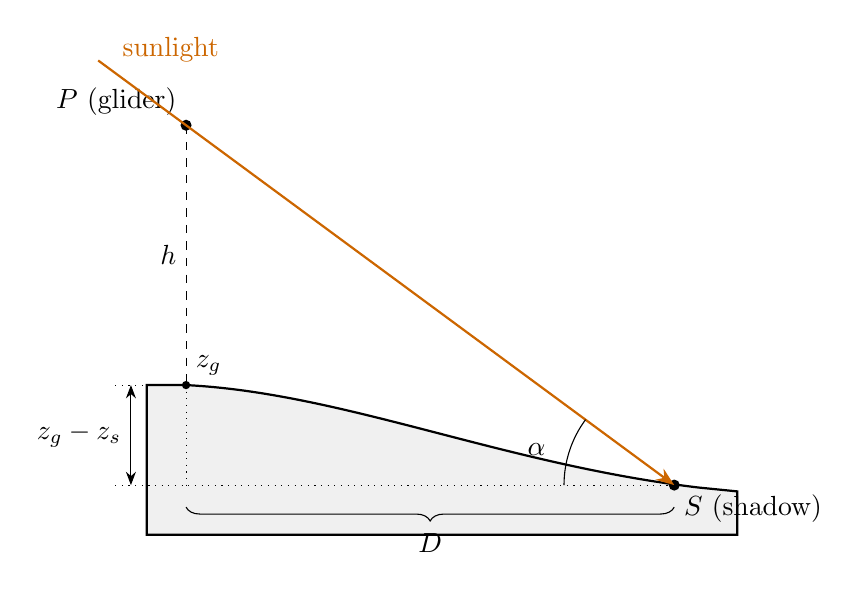
\begin{tikzpicture}[scale=1.0, >=Stealth]
  % terrain
  \draw[thick, fill=black!6] (-0.5,1.6) -- (0,1.6) .. controls (2,1.5) and (4,0.6) .. (6.5,0.3) -- (7,0.25) -- (7,-0.3) -- (-0.5,-0.3) -- cycle;
  % glider
  \coordinate (P) at (0,4.9);
  \coordinate (G) at (0,1.6);
  \coordinate (S) at (6.2,0.33);
  \fill (P) circle (2pt) node[above left] {$P$ (glider)};
  \fill (S) circle (2pt) node[below right] {$S$ (shadow)};
  \draw[dashed] (P) -- (G) node[midway, left] {$h$};
  \fill (G) circle (1.5pt) node[above right] {$z_g$};
  % sun ray
  \draw[->, thick, orange!80!black] ($(P)!-0.18!(S)$) -- (S);
  \node[orange!80!black, above right] at ($(P)!-0.15!(S)$) {sunlight};
  % horizontal through S and vertical through P
  \draw[dotted] (-0.9,0.33) -- (S);
  \draw[decorate, decoration={brace, amplitude=5pt, mirror}] (0,0.05) -- (6.2,0.05) node[midway, below=6pt] {$D$};
  \draw[dotted] (G) -- (0,0.33);
  \draw[dotted] (-0.9,1.6) -- (G);
  \draw[<->] (-0.7,0.33) -- (-0.7,1.6) node[midway, left] {$z_g - z_s$};
  % angle
  \draw ($(S)+(-1.4,0)$) arc[start angle=180, end angle={180-36.4}, radius=1.4];
  \node at ($(S)+(-1.75,0.45)$) {$\alpha$};
\end{tikzpicture}
\caption{Vertical section along the sunlight direction. On sloping terrain the
shadow falls lower than the ground beneath the glider ($z_s<z_g$). The terrain
difference therefore has to be removed from the height obtained along the ray.}
\label{fig:section}
\end{figure}

\subsection{Height above ground}

The height above the terrain directly beneath the glider is $h = Z - z_g$, where
$z_g$ is the terrain elevation at $(E_g,N_g)$. Eliminating $Z$ with
\eqref{eq:ray} gives the central formula
\begin{equation}
  \boxed{\,h = D\tan\alpha + z_s - z_g\,}
  \label{eq:height}
\end{equation}
The term $z_s - z_g$ is the terrain correction. A shadow that falls downhill
($z_s<z_g$) would overstate the height if the correction were ignored, and one that
falls uphill would understate it. On flat ground \eqref{eq:height} reduces to
$h = D\tan\alpha$.

The height is referred to the terrain directly beneath the glider, which is what
\emph{above ground level} means. If the height is wanted above some other reference,
such as the shadow point or sea level, replace $z_g$ in \eqref{eq:height}
with that reference.

\section{Solar elevation from reference masts}\label{sec:masts}

\subsection{Calibration equation}

A vertical mast of height $H$, with base elevation $z_b$, casts its top's shadow
at horizontal distance $L$ from the base, onto terrain at elevation $z_t$.
Applying \eqref{eq:ray} to the mast top gives
\begin{equation}
  \tan\alpha = \frac{H + z_b - z_t}{L}.
  \label{eq:mast}
\end{equation}
Substituting \eqref{eq:mast} into \eqref{eq:height} gives a combined estimator,
\begin{equation}
  h = \frac{D}{L}\,(H + z_b - z_t) + z_s - z_g .
  \label{eq:ratio}
\end{equation}
In \eqref{eq:ratio} the horizontal lengths enter only as the ratio $D/L$.
A scale error common to both, such as a wrong image resolution, therefore
cancels. This holds only if the mast and glider were imaged under the same sun.
Rays are parallel only at a single instant, so the mast shadow and the glider shadow
must come from the same exposure, or at least from exposures taken within minutes of
each other. Tiles of the same mosaic year do not establish this.

The mast top must be a point vertically above the base used for $z_b$. A point on
an offset crossarm needs its own horizontal projection. A second mast gives an
independent value of $\alpha$. The calculator compares it with the first value
and does not average the two. Averaging would hide a disagreement that may point to
a wrong shadow identification or to different capture times.

\subsection{Mast heights from ground photographs}\label{sec:streetview}

No surveyed mast heights were available. Each height was reconstructed from a
March~2011 ground panorama by elevation-angle triangulation.
The camera stands at terrain elevation $z_c$ with lens height $\ell$ above it and
horizontal distance $d$ from the mast. If the mast top is seen at angle $\beta$
above the horizontal,
\begin{equation}
  H = z_c + \ell + d\tan\beta - z_b .
  \label{eq:streetview}
\end{equation}

\begin{table}[ht]
\centering
\begin{tabular}{@{}lrr@{}}
\toprule
Input & Mast 1 & Mast 2 \\
\midrule
Terrain at camera $z_c$ & \SI{1790.3}{m} & \SI{1776.1}{m} \\
Assumed lens height $\ell$ & \SI{2.5}{m} & \SI{2.5}{m} \\
Horizontal distance $d$ & \SI{24.75}{m} & \SI{40.84}{m} \\
Top elevation angle $\beta$ & \ang{7.8} & \ang{17.4} \\
Terrain at mast base $z_b$ & \SI{1787.2}{m} & \SI{1781.4}{m} \\
\midrule
$H$ from \eqref{eq:streetview} & \SI{8.99}{m} & \SI{10.00}{m} \\
$\partial H/\partial\beta = d\sec^2\beta$ & \SI{0.44}{m/\degree} & \SI{0.78}{m/\degree} \\
Working bound & $\pm\SI{3}{m}$ & $\pm\SI{3}{m}$ \\
\bottomrule
\end{tabular}
\caption{Street-View reconstruction of the mast heights. The lens height is an
assumption: $\partial H/\partial\ell = 1$, so it passes one-for-one into $H$.
The $\pm\SI{3}{m}$ figure is a working sensitivity bound, not a measured tolerance.}
\label{tab:masts}
\end{table}

\subsection{How mast errors propagate}

From \eqref{eq:ratio}, $\partial h/\partial H = D/L = \tan\alpha \cdot D/(H+z_b-z_t)$.
Near $\alpha\approx\ang{65}$ a \SI{9}{m} mast on level ground casts a shadow of only
$L\approx\SI{4.2}{m}$. The amplification factor is then $D/L\approx18$, so a
\SI{\pm 3}{m} uncertainty in $H$ spreads the glider height over roughly
\SIrange{88}{197}{m}. That spread comes before any error in $L$, which at
\SI{10}{cm} ground resolution is itself a few percent. Short shadows under a high
summer sun make mast calibration intrinsically weak for this scene. This motivates
the ephemeris route described next.

\section{Solar elevation from an ephemeris}\label{sec:ephemeris}

\subsection{Acquisition time}

The covering SWISSIMAGE flight strip is \code{20230714\_1118\_12504}, flown on
14~July~2023. Its identifier encodes the \emph{start} of acquisition, 11:18~UTC.
The exposure at the glider comes later along the strip and is not published, so
the solar angle has to be bounded over a time window rather than evaluated at one
instant. The strip's whole extent is about \SI{58}{km} east–west. At typical
survey speeds that takes on the order of a quarter of an hour, and we adopt the
generous window 11:18--11:48~UTC.

\subsection{Solar position}

The solar position follows the low-precision algorithm of Meeus, as used in the
NOAA solar calculator, which is accurate to about \ang{;1;} for present-day dates.
With $T$ the number of Julian centuries since J2000.0, the steps are as follows:
\begin{align}
  L_0 &= \ang{280.46646} + \ang{36000.76983}\,T + \ang{0.0003032}\,T^2
     &&\text{(mean longitude)}\\
  M &= \ang{357.52911} + \ang{35999.05029}\,T - \ang{0.0001537}\,T^2
     &&\text{(mean anomaly)}\\
  \lambda &= L_0 + C(M) - \ang{0.00569} - \ang{0.00478}\sin\Omega
     &&\text{(apparent longitude)}\\
  \sin\delta &= \sin\varepsilon\,\sin\lambda
     &&\text{(declination)}
\end{align}
Here $C$ is the equation of centre, $\Omega$ the longitude of the Moon's
ascending node and $\varepsilon$ the obliquity of the ecliptic. The local hour angle
$H_\odot$ follows from UTC, the equation of time and the longitude $\lambda_{\mathrm{geo}}$.
With latitude $\varphi$, elevation and azimuth are
\begin{align}
  \sin\alpha &= \sin\varphi\sin\delta + \cos\varphi\cos\delta\cos H_\odot,
  \label{eq:elev}\\
  A_\odot &= \operatorname{atan2}\!\bigl(\sin H_\odot,\;
             \cos H_\odot\sin\varphi - \tan\delta\cos\varphi\bigr) + \ang{180}.
\end{align}
At the glider ($\varphi=\ang{46.3674}$\,N, $\lambda_{\mathrm{geo}}=\ang{7.2103}$\,E,
converted from LV95 with the swisstopo approximation and cross-checked against
the swisstopo REFRAME service), the declination is $\delta=\ang{21.68}$, the
equation of time is \SI{-5.9}{min}, and local solar noon falls at 11:37~UTC.

\begin{table}[ht]
\centering
\begin{tabular}{@{}lrrr@{}}
\toprule
UTC (2023-07-14) & $\alpha$ & $A_\odot$ & $\tan\alpha$ \\
\midrule
11:00 & \ang{64.19} & \ang{159.92} & 2.0676 \\
11:18 (strip start) & \ang{65.01} & \ang{169.49} & 2.1452 \\
11:24 & \ang{65.16} & \ang{172.74} & 2.1600 \\
11:37 (solar noon) & \ang{65.31} & \ang{179.98} & 2.1748 \\
11:48 & \ang{65.21} & \ang{186.08} & 2.1647 \\
12:18 & \ang{63.94} & \ang{202.09} & 2.0446 \\
\bottomrule
\end{tabular}
\caption{Solar position at the glider. An independent evaluation with
\textsc{astropy} agrees to within \ang{0.01} in both angles.}
\label{tab:sun}
\end{table}

Near solar noon $\dd\alpha/\dd t\approx 0$, so a modest error in the acquisition
time hardly affects the elevation. Over the whole window 11:18--11:48~UTC,
$\alpha\in[\ang{65.01},\,\ang{65.31}]$, i.e.\ $\alpha=\ang{65.16}\pm\ang{0.15}$.
In contrast, the azimuth turns at about \ang{0.5} per minute, which makes it a
sensitive clock (Section~\ref{sec:case}).

\section{Bounded uncertainty propagation}\label{sec:uncertainty}

\subsection{Interval arithmetic for monotone formulas}

Each input $x$ is given as a central value with a non-negative bound,
$x\in[x-\varepsilon_x,\,x+\varepsilon_x]$. The calculator reports the exact range of the
output over the box of all inputs. This is not a statistical confidence interval.

\begin{proposition}
Let $f(x_1,\dots,x_n)$ be monotone in each argument over a box
$B=\prod_i[a_i,b_i]$. Then $\min_B f$ and $\max_B f$ are attained at the corner where
each $x_i$ is set to the end of its interval that minimises or maximises $f$. That
end is fixed by the sign of $\partial f/\partial x_i$.
\end{proposition}
\begin{proof}
Change one coordinate at a time towards the chosen endpoint. By monotonicity no
step decreases (or increases) $f$, so the chosen corner is extremal.
\end{proof}

\noindent\emph{Height formula.} With $D>0$ and $\tan\alpha>0$, $h$ in
\eqref{eq:height} increases with $D$, $\tan\alpha$ and $z_s$ and decreases with $z_g$.
The terrain elevations $z_s$ and $z_g$ are bounded independently, each by
$\varepsilon_z$. Hence
\begin{align}
  h_{\min} &= (D-\varepsilon_D)\,\tan\alpha_{\min} + (z_s-z_g) - 2\varepsilon_z,\\
  h_{\max} &= (D+\varepsilon_D)\,\tan\alpha_{\max} + (z_s-z_g) + 2\varepsilon_z,
\end{align}
provided $D-\varepsilon_D>0$. Because $\tan$ is increasing on $(\ang{0},\ang{90})$,
a direct solar bound $\alpha\pm\varepsilon_\alpha$ maps to
$[\tan(\alpha-\varepsilon_\alpha),\tan(\alpha+\varepsilon_\alpha)]$.
The calculator requires $0<\alpha-\varepsilon_\alpha$ and
$\alpha+\varepsilon_\alpha<\ang{90}$.

\noindent\emph{Mast calibration.} Write $R=H+z_b-z_t$ for the rise.
Then $\tan\alpha=R/L$ increases in $R$ and decreases in $L$, and
$\varepsilon_R=\varepsilon_H+2\varepsilon_z$, so
\begin{equation}
  \tan\alpha_{\min} = \frac{R-\varepsilon_R}{L+\varepsilon_L},\qquad
  \tan\alpha_{\max} = \frac{R+\varepsilon_R}{L-\varepsilon_L},
\end{equation}
which require $R-\varepsilon_R>0$ and $L-\varepsilon_L>0$. These conditions mean the
Sun must stay above the horizon and the shadow must have positive length throughout
the box. Chaining the two monotone maps gives the overall height interval.

The worst case treats $z_s$, $z_g$ (and $z_b$, $z_t$) as independent. If their
errors are correlated, for example through a common datum offset, the true spread is
smaller, so the interval is conservative. Bounds set to zero mean that the
uncertainty is \emph{not quantified}, not that the input is exact.

\subsection{First-order sensitivities}

Linearising \eqref{eq:height} shows which input dominates:
\begin{equation}
  \frac{\partial h}{\partial D} = \tan\alpha,\qquad
  \frac{\partial h}{\partial\alpha} = D\sec^2\alpha,\qquad
  \frac{\partial h}{\partial z_s} = 1,\qquad
  \frac{\partial h}{\partial z_g} = -1.
\end{equation}
At $\alpha=\ang{65.16}$, $\tan\alpha=2.16$ and $\sec^2\alpha=5.66$. For $D=\SI{76}{m}$:
\begin{itemize}
  \item \SI{1}{m} of horizontal error in $D$ moves $h$ by \SI{2.16}{m};
  \item \ang{1} of solar error moves $h$ by $D\sec^2\alpha\cdot\pi/180=\SI{7.5}{m}$;
  \item each metre of terrain error moves $h$ by \SI{1}{m}.
\end{itemize}
A high Sun amplifies errors in the measured separation. Accuracy therefore depends
on locating the glider and its shadow correctly far more than on the exact timestamp.

\section{Error sources outside the bounds}\label{sec:systematic}

\subsection{Orthophoto displacement of the glider}

The orthophoto places every pixel as if it lay on the terrain. A point at height
$h$ above the terrain, viewed at zenith angle $\theta$ from the camera, is therefore
drawn displaced \emph{away} from the camera's nadir by
\begin{equation}
  \Delta = h\tan\theta .
  \label{eq:relief}
\end{equation}
The shadow lies on the terrain and is not displaced. Only the component of
$\Delta$ along the shadow direction changes $D$. Let $\theta_\parallel$ be the
signed view tilt projected onto the vertical plane of the sunlight, positive when
the glider is drawn towards its shadow. The observed separation is then
$D_{\mathrm{obs}} = D - h\tan\theta_\parallel$. Substituting
$D = D_{\mathrm{obs}} + h\tan\theta_\parallel$ into \eqref{eq:height} and solving for $h$
gives the self-consistent correction
\begin{equation}
  h = \frac{D_{\mathrm{obs}}\tan\alpha + z_s - z_g}{1-\tan\theta_\parallel\tan\alpha}.
  \label{eq:relief-corrected}
\end{equation}
The amplification is strong. With $\tan\alpha\approx2.16$, a view tilt of only
\ang{\pm5} along the ray changes $h$ by roughly \SIrange{-16}{+23}{\percent}. That is
about \SIrange{-23}{+33}{m} at $h\approx\SI{142}{m}$.
The camera pose of the source exposure is not reconstructed here,
so $\theta_\parallel$ is unknown. Equation~\eqref{eq:relief-corrected} is the
place to apply it once it is known. The calculator uses the apparent glider
position and flags its results as provisional for this reason. The terrain value
$z_g$ should also be re-read beneath the corrected glider position.

The displacement component \emph{perpendicular} to the shadow ray would show up as
a mismatch between the observed azimuth $A_{gs}$ and $A_\odot+\ang{180}$ at the
exposure time. Section~\ref{sec:case} finds no such mismatch within the time
window. The along-ray component, which is the one that affects $h$, cannot be
detected that way.

\subsection{Other effects}
\begin{itemize}
  \item \textbf{Finite solar disk.} The Sun subtends $\approx\SI{9.3}{mrad}$, so a
        shadow cast from slant range $h/\sin\alpha$ is blurred by about
        \SI{1.6}{m} along the ground. This softens the shadow edges but leaves the centroid
        unbiased. Matching corresponding points (e.g.\ wing centre to shadow centre)
        avoids edge bias.
  \item \textbf{Shadow identification.} If the shadow belongs to a different
        object or a different exposure, the result is meaningless. No interval
        covers this.
  \item \textbf{Mosaic time mixing.} A mosaic may combine exposures taken at
        different times. Mast calibration is valid only if masts and glider share
        one exposure.
  \item \textbf{Terrain epoch and surface.} The terrain service reflects the present
        bare-earth model, not necessarily the surface at acquisition (snow,
        vegetation, works).
\end{itemize}

\section{Case study: Isenau, 14 July 2023}\label{sec:case}

\begin{table}[ht]
\centering
\begin{tabular}{@{}lrrr@{}}
\toprule
Point & Easting & Northing & Terrain \\
\midrule
Glider (apparent) & \num{2582425.46} & \num{1135134.94} & \SI{1927.8}{m} \\
Shadow (candidate) & \num{2582415.86} & \num{1135210.29} & \SI{1906.4}{m} \\
\bottomrule
\end{tabular}
\caption{LV95 coordinates of the map pins and terrain elevations (retrieved
7~October~2026). These are pin centres, not surveyed points.}
\label{tab:inputs}
\end{table}

\paragraph{Geometry.} From Table~\ref{tab:inputs},
$D=\SI{75.959}{m}$, $A_{gs}=\ang{352.74}$ and $z_s-z_g=\SI{-21.4}{m}$. The shadow
falls about \SI{21}{m} downhill, so the terrain correction lowers the height.

\paragraph{Azimuth consistency.} Equation~\eqref{eq:azimuth} requires
$A_\odot = \ang{172.74}$, which the ephemeris gives at 11:24~UTC. That is six minutes
after the strip start and inside the adopted window. The shadow direction is
therefore consistent with the documented flight, and there is no evidence of a
cross-ray displacement. A shadow cast an hour earlier or later would point about \ang{30} away.

\paragraph{Height (ephemeris route).} With $\alpha=\ang{65.16}\pm\ang{0.15}$ and
the apparent glider position,
\begin{equation}
  h = 75.959\times\tan\ang{65.16} - 21.4 \approx \SI{142.7}{m},
  \qquad h\in[\SI{141.5}{m},\,\SI{143.8}{m}]
  \ \text{(solar bound only)}.
\end{equation}
Adding plausible measurement bounds of $\varepsilon_D=\SI{5}{m}$ and
$\varepsilon_z=\SI{1}{m}$ widens this to \SIrange{128.8}{156.7}{m}. Even a
$\pm\ang{1}$ solar bound, wide enough to cover acquisition anywhere from about
11:00 to 12:15~UTC, gives \SIrange{135.4}{150.5}{m} with exact $D$ and terrain.

\paragraph{Height (mast route).} The aerial shadow lengths of the two masts have
not yet been measured. The mast route therefore yields no number, and with
$\pm\SI{3}{m}$ mast heights it would be much weaker than the ephemeris
(Section~\ref{sec:masts}). Measured mast shadows remain valuable as an
independent check that the solar angle in the actual exposure is about \ang{65}.

\paragraph{Summary.} Taking the apparent glider position, the candidate shadow
and the documented flight date, the glider was about $\SI{140}{m}$ above the
terrain beneath it. The result is conditional on:
\begin{enumerate}[label=(\roman*)]
  \item correct shadow identification;
  \item exposure during the 2023-07-14 strip near midday;
  \item a negligible along-ray orthophoto displacement.
\end{enumerate}
Condition (iii) is the one that limits the accuracy. Equation~\eqref{eq:relief-corrected}
shows how to correct for it once the source exposure geometry is known.

\section{Implementation and verification}

\begin{table}[ht]
\centering
\begin{tabular}{@{}ll@{}}
\toprule
Equation & Implementation \\
\midrule
\eqref{eq:ray}, \eqref{eq:azimuth} & \code{separation()} \\
\eqref{eq:mast} + bounds & \code{calibrateReference()} \\
direct $\alpha\pm\varepsilon_\alpha$ & \code{directSun()} \\
\eqref{eq:height} + bounds & \code{heightFromShadow()} \\
whole pipeline, warnings & \code{solve()} \\
\eqref{eq:elev} ff., LV95$\to$WGS84 & \code{paper/solar.mjs} \\
\bottomrule
\end{tabular}
\caption{Where each equation is implemented. Functions without a path are in
\code{glider-height/dist/calculations.mjs}.}
\end{table}

The calculation module has no dependencies. Its test suite (\code{npm test} in
\code{glider-height/}) checks the following:
\begin{itemize}
  \item the LV95 separation and azimuth of the case-study pins;
  \item $h=D$ on flat ground at \ang{45};
  \item the sign of the uphill and downhill corrections;
  \item the corner-case interval bounds against hand-computed values;
  \item rejection of non-finite, singular and horizon-grazing inputs;
  \item non-averaging of the second mast;
  \item flagging, rather than clamping, of below-ground results.
\end{itemize}
The solar positions in Table~\ref{tab:sun} were cross-checked against
\textsc{astropy} (agreement better than \ang{0.01}). The coordinate conversion was
cross-checked against the swisstopo REFRAME service (agreement better than
\SI{1}{m}).

\section*{Data sources}
{\raggedright
\begin{itemize}
  \item swisstopo SWISSIMAGE orthophoto mosaic, and flight-strip metadata for
        strip \code{20230714\_1118\_12504} from the layer
        \nolinkurl{ch.swisstopo.lubis-bildstreifen}.
  \item swisstopo swissALTI3D terrain model via the geo.admin.ch height service.
  \item Ground panoramas (March 2011) for the mast-height reconstruction; linked,
        not reproduced.
  \item J.~Meeus, \emph{Astronomical Algorithms}, 2nd ed., Willmann-Bell, 1998;
        NOAA Global Monitoring Laboratory solar calculator.
\end{itemize}
}

\end{document}
